\documentclass[11pt]{article}

% some definitions for the title page
\newcommand{\reporttitle}{example}
\newcommand{\reportdescription}{example description}

% load some definitions and default packages
%---------------------------------------------------------------------------
%	PACKAGES AND OTHER DOCUMENT CONFIGURATIONS
%---------------------------------------------------------------------------

\usepackage[twoside]{fancyhdr}
\usepackage{csquotes}

\usepackage[a4paper,hmargin=2.0cm,vmargin=1.0cm,includeheadfoot]{geometry}
% \usepackage{natbib} % for bibliography
\usepackage{biblatex}
\usepackage{tabularx,longtable,multirow,subfigure,caption}%hangcaption
\usepackage{fancyhdr} % page layout
\usepackage{url} % URLs
\usepackage[english]{babel}
\usepackage{graphicx}
\usepackage{rotating}
\usepackage{dsfont}
\usepackage{epstopdf} % automatically replace .eps with .pdf in graphics
% \usepackage{backref} % needed for citations
\usepackage{array}
\usepackage{latexsym}
\usepackage[pdftex,hypertexnames=false,colorlinks]{hyperref} % provide links in pdf (had pagebackref)
\usepackage{booktabs}
\usepackage{wrapfig}
\usepackage{caption}  % Required for \captionof
\usepackage{float} % for H option in figures
\usepackage{amssymb}
\usepackage{amsmath}
\usepackage{amsthm}
\usepackage{mathtools} % for 'dcases*' env.
\usepackage[nottoc]{tocbibind}

%%% Default fonts
\renewcommand*{\rmdefault}{bch}
\renewcommand*{\ttdefault}{cmtt}

%%% Default settings (page layout)
\setlength{\parindent}{0em}  % indentation of paragraph
\setlength{\parskip}{.3em}
\setlength{\itemsep}{0.mm}

\setlength{\headheight}{14.5pt}
\pagestyle{fancy}

\fancyfoot[ER,OL]{\thepage}%Page no. in the left on odd pages and on right on even pages

\fancyfoot[OC,EC]{\sffamily }
\renewcommand{\headrulewidth}{0.1pt}
\renewcommand{\footrulewidth}{0.1pt}
\captionsetup{margin=10pt,font=small,labelfont=bf}

% LISTINGS ammendments
\usepackage{listings}
\usepackage{color}

\definecolor{mygreen}{rgb}{0,0.6,0}
\definecolor{mygray}{rgb}{0.5,0.5,0.5}
\definecolor{mymauve}{rgb}{0.58,0,0.82}

\lstset{ 
  postbreak=\mbox{\textcolor{red}{$\hookrightarrow$}\space},
  backgroundcolor=\color{white},   % choose the background color; you must add \usepackage{color} or \usepackage{xcolor}; should come as last argument
  basicstyle=\footnotesize,        % the size of the fonts that are used for the code
  breakatwhitespace=false,         % sets if automatic breaks should only happen at whitespace
  breaklines=true,                 % sets automatic line breaking
  captionpos=b,                    % sets the caption-position to bottom
  commentstyle=\color{mygreen},    % comment style
%   deletekeywords={...},            % if you want to delete keywords from the given language
%   escapeinside={\%*}{*)},          % if you want to add LaTeX within your code
  extendedchars=true,              % lets you use non-ASCII characters; for 8-bits encodings only, does not work with UTF-8
  firstnumber=1,                % start line enumeration with line 1000
  frame=single,	                   % adds a frame around the code
  keepspaces=true,                 % keeps spaces in text, useful for keeping indentation of code (possibly needs columns=flexible)
  columns=fullflexible,
  keywordstyle=\color{blue},       % keyword style
  language=python,                 % the language of the code
  % morekeywords={*,...},            % if you want to add more keywords to the set
  numbers=left,                    % where to put the line-numbers; possible values are (none, left, right)
  numbersep=5pt,                   % how far the line-numbers are from the code
  numberstyle=\tiny\color{mygray}, % the style that is used for the line-numbers
  rulecolor=\color{black},         % if not set, the frame-color may be changed on line-breaks within not-black text (e.g. comments (green here))
  showspaces=false,                % show spaces everywhere adding particular underscores; it overrides 'showstringspaces'
  showstringspaces=false,          % underline spaces within strings only
  showtabs=false,                  % show tabs within strings adding particular underscores
  stepnumber=1,                    % the step between two line-numbers. If it's 1, each line will be numbered
  stringstyle=\color{mymauve},     % string literal style
  tabsize=2,	                   % sets default tabsize to 2 spaces
  title=\lstname% show the filename of files included with \lstinputlisting; also try caption instead of title
}

% Here, you can define your own macros. Some examples are given below.

\newcommand{\R}[0]{\mathds{R}} % real numbers
\newcommand{\Z}[0]{\mathds{Z}} % integers
\newcommand{\N}[0]{\mathds{N}} % natural numbers
\newcommand{\C}[0]{\mathds{C}} % complex numbers
\renewcommand{\vec}[1]{{\boldsymbol{{#1}}}} % vector
\newcommand{\mat}[1]{{\boldsymbol{{#1}}}} % matrix


\bibliography{../bibliography}

\begin{document}

% Include the title page
\begin{titlepage}

    \newcommand{\HRule}{\rule{\linewidth}{0.5mm}} % Defines a new command for the horizontal lines, change thickness here
    
    \center % Center everything on the page
     
    %------------------------------------------------------------------------
    %	HEADING SECTIONS
    %------------------------------------------------------------------------
    
    \textsc{\Large Department of Computing}\\[0.5cm] 
    \textsc{\large Imperial College of Science, Technology and Medicine}\\[0.5cm] 
    
    %------------------------------------------------------------------------
    %	TITLE SECTION
    %------------------------------------------------------------------------
    
    \HRule \\[0.4cm]
    { \huge \bfseries \reporttitle}\\ % Title of your document
    \HRule \\[0.4cm]

    \textit{\reportdescription}
    
    \vspace{2em}

    %------------------------------------------------------------------------
    %	AUTHOR SECTION
    %------------------------------------------------------------------------
    
    \large \emph{Author: Anton Zhitomirskiy}

    \vspace{1em}

    \global\let\newpagegood\newpage
    \global\let\newpage\relax
    
\end{titlepage}

\global\let\newpage\newpagegood

\tableofcontents

\clearpage

\section{Semantic Segmentation}

\begin{figure}[H]
    \centering
    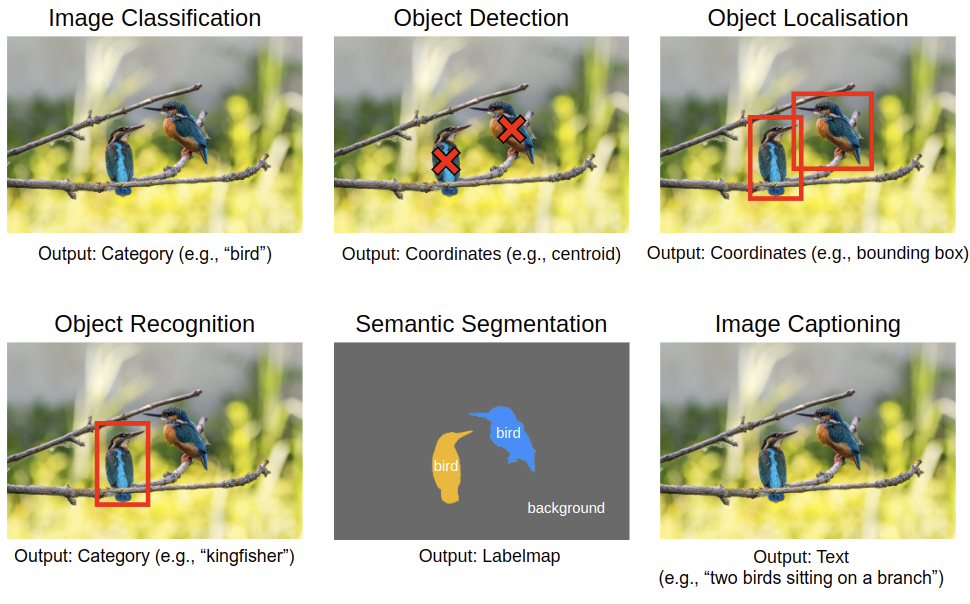
\includegraphics[width=.9\linewidth]{figures/common-image-analysis-tasks.png}
    \caption{Common image analysis tasks}
\end{figure}

\begin{definition}[Semantic Segmentation]
    Given an input image, we want to label individaul pixels in the image accroding to which object or class they blong to. It is a dense classification where every pixel is being assigned to a specific class.

    Each segmented region is assigned a semantic meaning (which contrasts the segmentation based on `pure' clustering of the image into coherent regions).
\end{definition}

\subsection{Uses}

\begin{itemize}
    \item conducting quantitative analysis, e.g. measuring the volume of a ventricular cavity
    \item determining the precise location and extent of an organ or certain type of tissue, e.g. a tumour, for treatment such as radiation therapy
    \item creating 3D models used for simulation, e.g. genrating a model of an abdominal aortic aneurysm for simulating stress/strain distributions
\end{itemize}

\section{Challenges}

\subsection{noise}

Noise in images refers to high-frequency pixel variability which is not relevant, or may obscure, the model's task.

\subsection{partical volume effects}

The image produced by software is a quantized version of the object. Due to the coarse sampling, the resulting image shows partial volume effects at the boundary of the image. These pixels are not aligned with real world boundaries. Therefore, the pixels contain a mixture of two different objects.

An object may also be elevated, and it is therefore difficult to measure where the extent of the obejct is because it is unclear where the object starts or ends.

\begin{figure}[H]
    \centering
    \subfigure[Pixel mixing between boundaries]{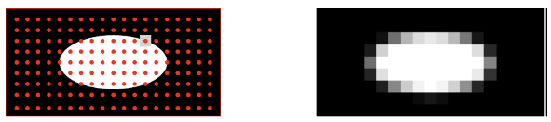
\includegraphics[width=\linewidth]{figures/partial-volume-effect.png}}
    \subfigure[Elevated region]{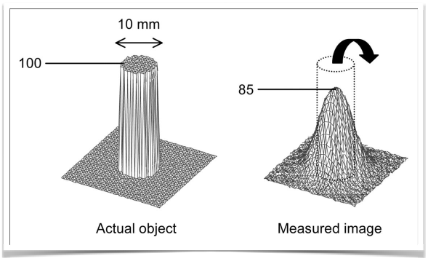
\includegraphics[width=.4\linewidth]{figures/elevated-region-volume-effect.png}}
    \caption{Partial volume effects}
\end{figure}

\subsection{Intensity Inhomogeneities}

You have the problem that ou might have varying contrast and intensity differences across the image plain. In an ultrasound, the images are acquired from a sensor that sends ultrasound waves into the body so that they may be absorbed by the tissue. This causes lower levels to appear darker on the scan. However, the further down you go, the less signal you get back. Similarly, in an MRI we also have contrasting areas accross the iamge.

\subsection{Anisostropic Resolution}

Often 2D stacks (x-y dimension) will have high resolution, however, in the z dimension the resolution may be larger, which causes less clarity when looking along this view.

\begin{figure}[H]
    \centering
    \subfigure[An MRI acquisition of short axis slices of the left ventricle may have an intraslice resolution of 1.3mm and an interslice resolution of 8mm]{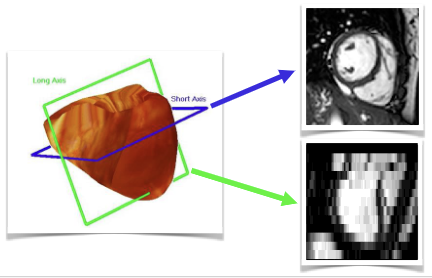
\includegraphics[width=.4\linewidth]{figures/anisotropic-resolution.png}}
    \subfigure[Anisotropic resolution with french-fry boxes]{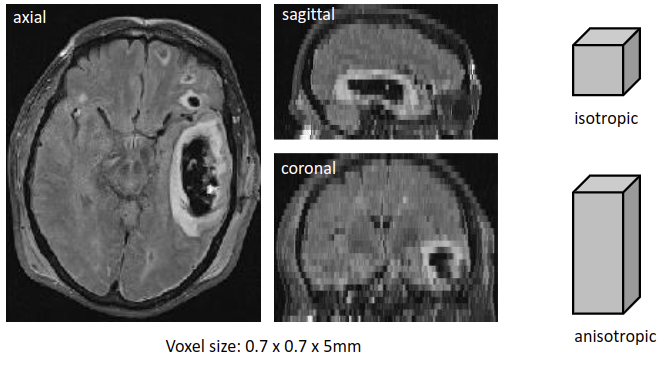
\includegraphics[width=.4\linewidth]{figures/anisotropic-resolution-2.png}}
\end{figure}

\subsection{Imaging Artifacts}

\begin{figure}[H]
    \centering
    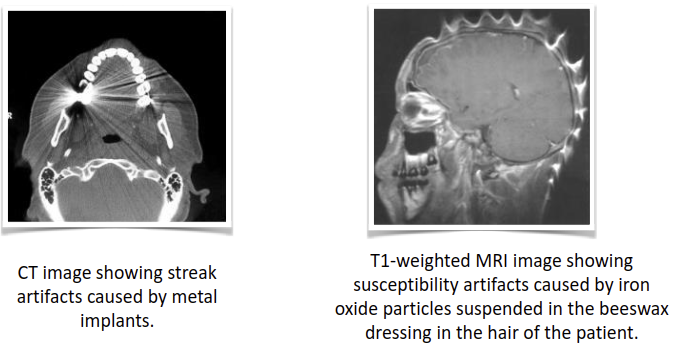
\includegraphics[width=.4\linewidth]{figures/image-artifact.png}
    \caption{Image artifacts}
\end{figure}

\subsection{limited contrasts}

Different tissues can have simlar physical properties and thus similar intesity values. Purely intensity-based algorithms are prone to fail or ``leak'' into adjacent tissues.

\begin{figure}[H]
    \centering
    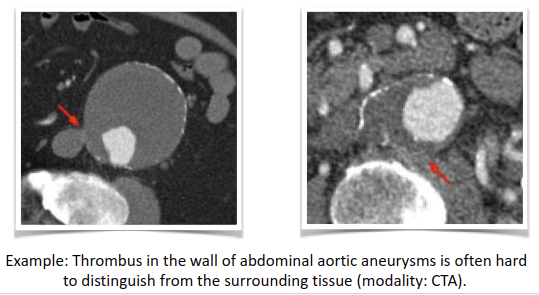
\includegraphics[width=.4\linewidth]{figures/limited-contrast.png}
    \caption{Limited contrast}
\end{figure}

\subsection{Morphological Variability}

There is variability between structures we want to segment. It makes it hard to incorporate meaningful prior information or useful shape models.

\begin{figure}[H]
    \centering
    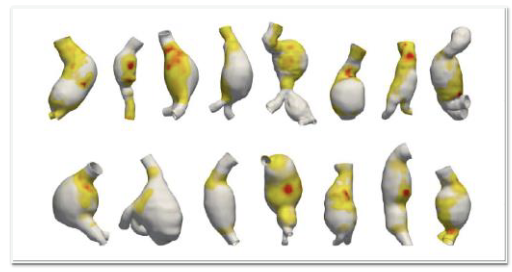
\includegraphics[width=.4\linewidth]{figures/morphological-variablity.png}
    \caption{Morphological variablity. A collectino of abdominal aortic aneurysms acquired with PET-CT and colored by FDG-18 uptake values}
\end{figure}

\section{Segmentation Evaluation}

\subsection{Ground truth}

\begin{definition}
    Reference or standard against which a method can be comapred, e.g. the otpimal transformation, or a true segmentaiton boundary.
\end{definition}

In practice, it is difficult to obtain. We can establish a ground truth with synthetically obtained data, for example, simulated phantoms or around structures we manufactured, such as gel phantoms.

\subsection{Gold standard}

Usually, an expert manually segments an image.

The disadvantage, is that it 

\begin{itemize}
    \item requires training and is a tedious and time-consuming process. 
    \item There is also intra-oberver variability (disagreement between same obserer on different occasions) 
    \item and inter-observer variability (disagreement between observers)
\end{itemize}

The remedy, is that

\begin{itemize}
    \item human observers can perform segmentation repeatedly. 
    \item Multiple experts can perform segmentations, 
    \item agreement or disagreement can be quantified 
\end{itemize}

\subsection{Evaluation Metrics}

\subsubsection{Precision}

\begin{figure}[H]
    \center
    \subfigure{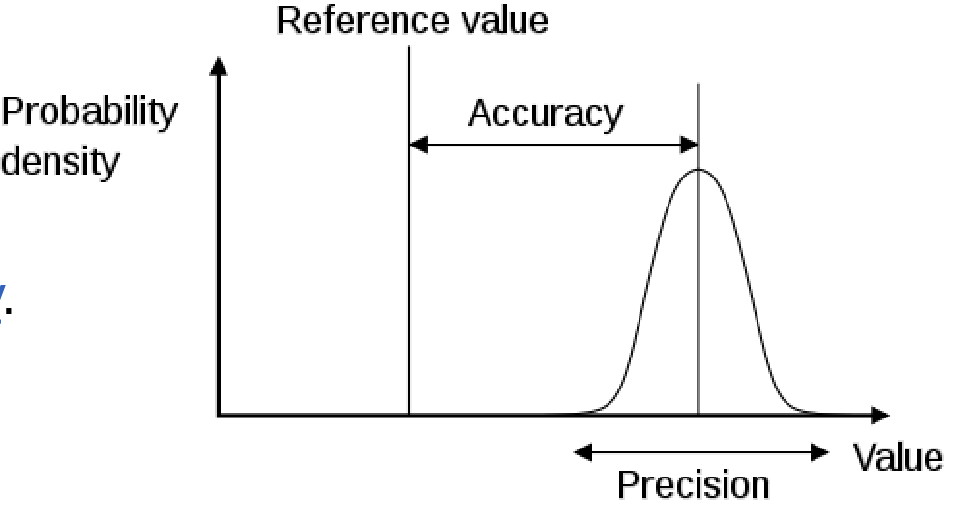
\includegraphics[width=0.4\textwidth]{figures/precision-accuracy.png}}
    \subfigure{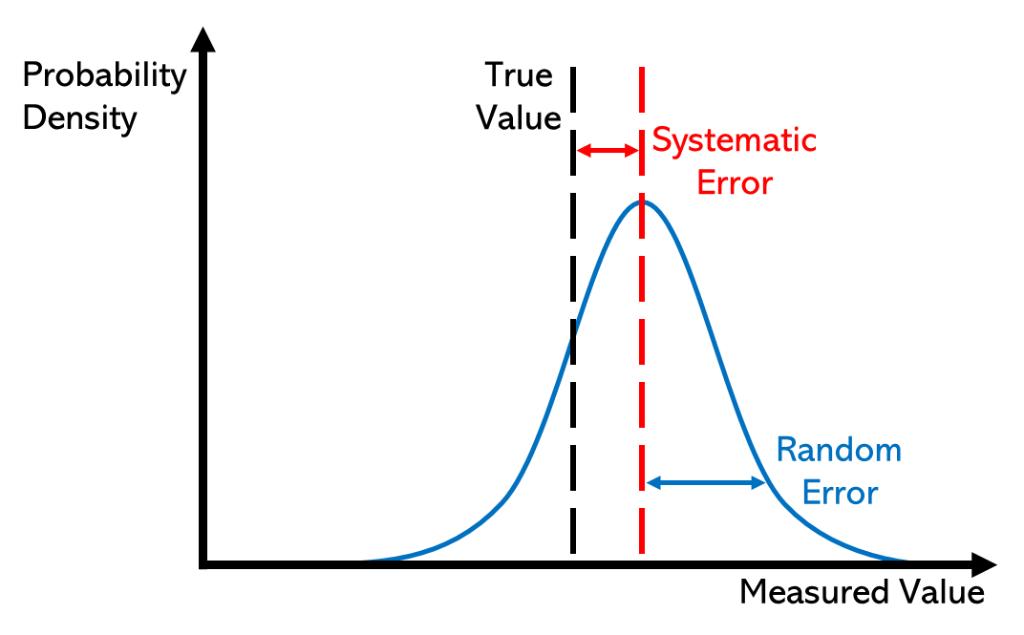
\includegraphics[width=0.4\textwidth]{figures/Measurement_distribution_with_systematic_and_random_errors.svg.png}}
\end{figure}


Is a description of \href{https://en.wikipedia.org/wiki/Observational_error}{random errors}, a measure of \href{https://en.wikipedia.org/wiki/Statistical_dispersion}{statistical variability}. It is the repeatbility or reproducibility of the measurement.

\subsubsection{Accuracy}

More commonly, it is a description of \href{https://en.wikipedia.org/wiki/Observational_error#Random_errors_versus_systematic_errors}{systematic errors}, a measure of \href{https://en.wikipedia.org/wiki/Bias_(statistics)}{statistical bias}; as these cause a difference between a result and a ``true'' value, \href{https://en.wikipedia.org/wiki/International_Organization_for_Standardization}{ISO} calls this \textit{trueness}.

Alternatively, ISO defines accuracy as describing a combination of both types of \href{https://en.wikipedia.org/wiki/Observational_error}{observational error} above (random and systematic), so high accuracy requires both high precision and high trueness.

\subsubsection{Robustness}

The degradation in performance with respect to varying noise levels or varying artefacts.

\subsubsection{Confusion matrix}

\begin{figure}[H]
    \centering
    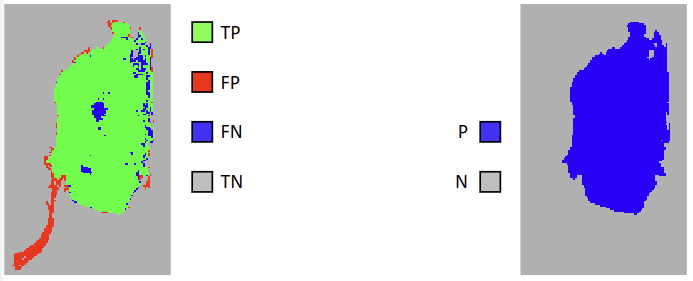
\includegraphics[width=.5\linewidth]{figures/confusion-matrix.png}
    \caption{confusion matrix with $TP$ true positive, $TN$ correct rejection, $FP$ false alarm, type I error, $FN$ miss, type II error. Also, $P$ is the number of real positive cases in the dataset, $N$ is the number of real negative cases in the data.}
\end{figure}

\subsubsection{Accuracy}

\begin{definition}[Accuracy]
    \begin{equation*}
        \frac{TP + TN}{P + N} = \frac{TP + TN}{(TP + FN) + (TN + FP)}
    \end{equation*}
\end{definition}

\subsubsection{Precision | positive predicttive value}

\begin{definition}[Precision]
    \begin{equation*}
        \frac{TP}{TP + FP}
    \end{equation*}
\end{definition}

\subsubsection{Recall | sensitivity | hit rate | true positive rate}

\begin{definition}[Recall]
    \begin{equation*}
        \frac{TP}{TP + FN}
    \end{equation*}
\end{definition}

\subsubsection{Specificity | True negative rate}

\begin{definition}[Specificity]
    \begin{equation*}
        \frac{TN}{N} = \frac{TN}{TN + FP} 
    \end{equation*}
\end{definition}

\subsubsection{F1 score}

\begin{definition}[F1 score]
    \begin{equation*}
        2\frac{Precision \cdot Recall}{Precision + Recall} = \frac{2TP}{2TP + FP + FN}
    \end{equation*}
\end{definition}

It is tough to use two metrics independently, it is the harmonic mean between the two.

\subsubsection{`IoU' - Overlap based - Jaccard Index}

\begin{definition}[Jaccard Index | Intersection over Union]
    \begin{equation*}
        \frac{|A\cap B|}{|A \cup B|}
    \end{equation*}
\end{definition}

\subsubsection{`DSC' - Overlap based - Dice Similarity}

The most widely used measure for evaluating segmentation. Assume that $A$ is the reference, and $B$ is the prediction. Therefore, with $|A| = TP + FN$ and $|B| = TP + FP|$, DSC is equivalent to F1.

\begin{definition}[DICE]
    \begin{equation*}
        2\frac{|A\cap B|}{|A|+|B|}
    \end{equation*}
\end{definition}

\subsubsection{Volume similarity}

\begin{definition}[Volume similarity]
    \begin{equation*}
        1 - \frac{||A| - |B||}{|A| + |B|} = 1 - \frac{|FN - FP|}{2TP + FP +F FN}
    \end{equation*}
\end{definition}

\subsubsection{`HD' - Surface Hasudorff distance}

\begin{figure}[H]
    \centering
    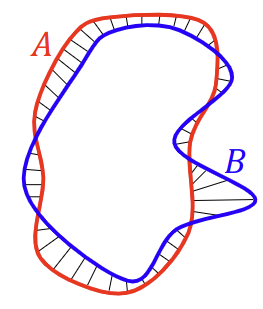
\includegraphics[width=.2\linewidth]{figures/Hausdorff.png}
\end{figure}

\begin{definition}[Hausdorff distance]
    \begin{equation*}
        \max(h(A,B),h(B,A)), \quad h(A,B) = \max_{a\in A} \min_{b\in B} ||a-b||
    \end{equation*}
\end{definition}

\subsubsection{`ASSD' - Surface (symmetric) average surface distance}

\begin{definition}[Average surface distance]
    \begin{equation*}
        ASD = \frac{d(A,B)+d(B,A)}{2}, \quad d(A,B)=\frac 1 N \sum_{a\ in A} \min_{b \in B} ||a - b||
    \end{equation*}
\end{definition}

\subsection{Pitfalls in segmentation evlauation}

``In a field such as athletics, this process is straightforward because the performance measurements (e.g., the time it takes an athlete to run a given distance) exactly reflect the underlying interest (e.g., which athlete runs a given distance the fastest?) [...] If the performance of an image analysis algorithm is not measured according to relevant validation metrics, no reliable statement can be made about the suitability of this algorithm in solving the proposed task, and the algorithm is unlikely to ever reach the stage of real-life application''~\cite{pitfalls-in-segmentation-evaluation}. 

\subsubsection{Effect of structure size}

``The Mask IoU (second column) is less sensitive to boundary errors for large objects. The Boundary IoU (third and fourth column) especially considers contours, (1) yields smaller metric scores, thus penalizing errors in the boundaries, and (2) is more invariant to structure sizes, leading to very similar values for large and small structures (fourth column). This pitfall is also relevant for other overlap-based metrics''~\cite{pitfalls-in-segmentation-evaluation}

\begin{figure}[H]
    \centering
    \subfigure{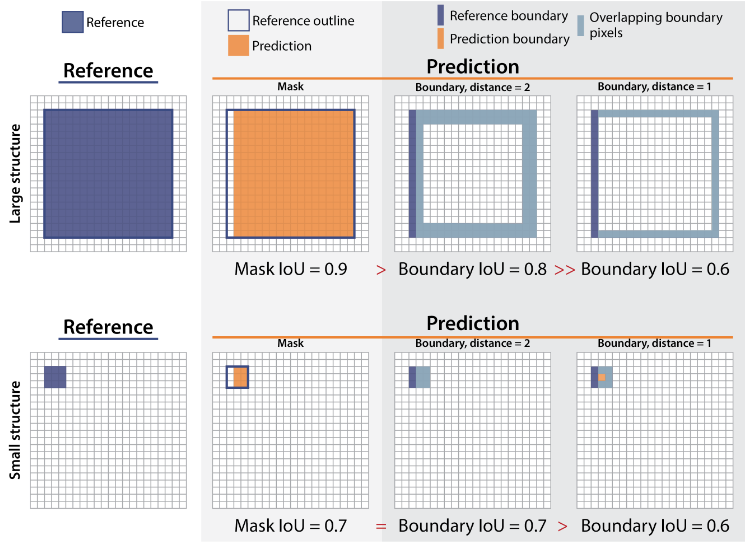
\includegraphics[width=.7\linewidth]{figures/size-0.png}}
    \caption{Extended Data Fig. SN 2.12~\cite{pitfalls-in-segmentation-evaluation}}
\end{figure}

``Large structures completely dominate overlap-based metrics in semantic segmentation problems. While Prediction 1 perfectly segments all three small structures, the metric score (here: Dice Similarity Coefficient ( DSC)) is much worse compared to the score of Prediction 2, with only one perfect prediction for the large structure. This is highlighted by only computing the metric without the large structure. This pitfall is also relevant for other overlap-based metrics.''~\cite{pitfalls-in-segmentation-evaluation}

\begin{figure}[H]
    \centering
    \subfigure{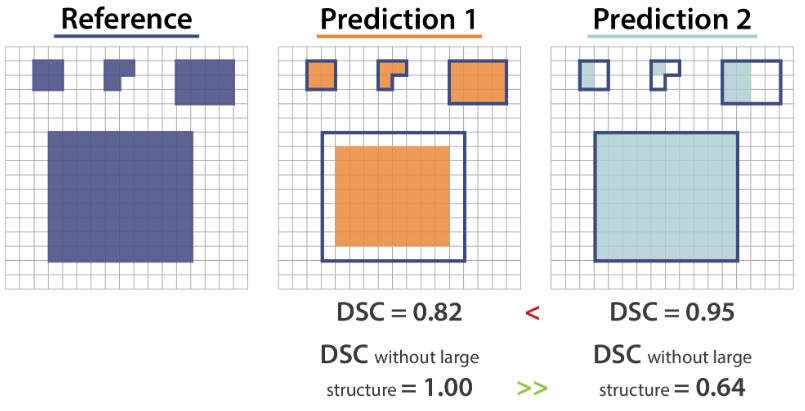
\includegraphics[width=.7\linewidth]{figures/size--1.png}}
    \caption{Extended Data Fig. SN 2.13~\cite{pitfalls-in-segmentation-evaluation}}
\end{figure}


% \subfigure{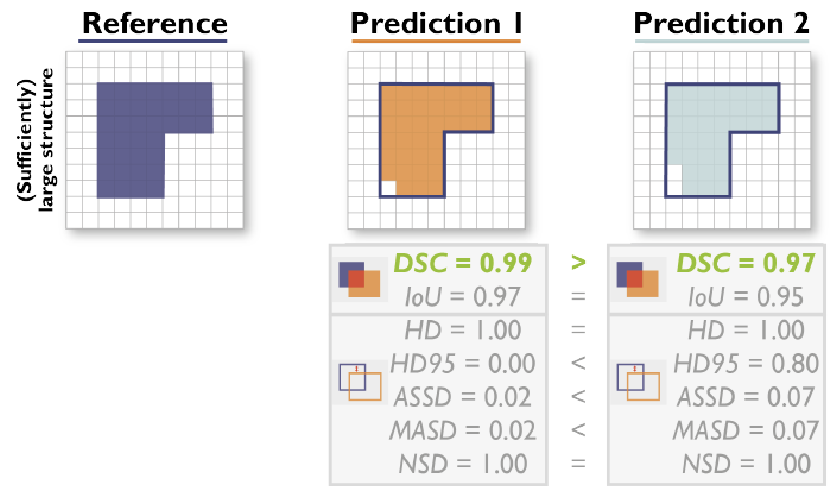
\includegraphics[width=.3\linewidth]{figures/size-a.png}}
\begin{figure}[H]
    \centering
    \subfigure{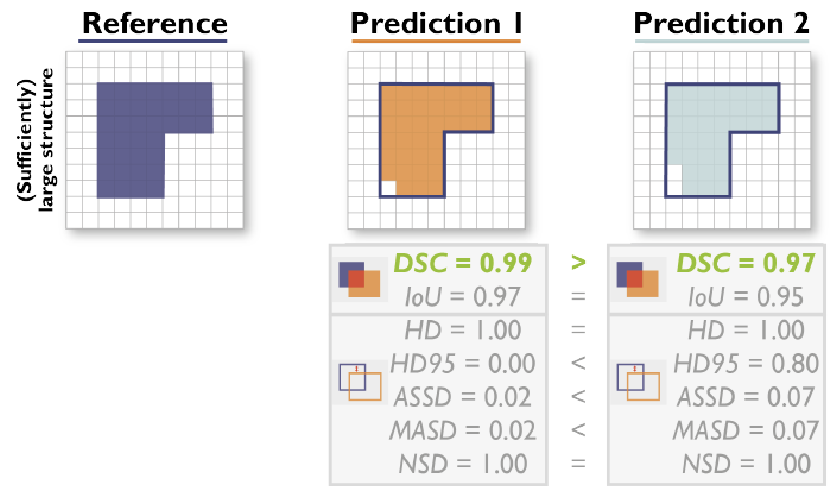
\includegraphics[width=.45\linewidth]{figures/size-a.png}}
    \subfigure{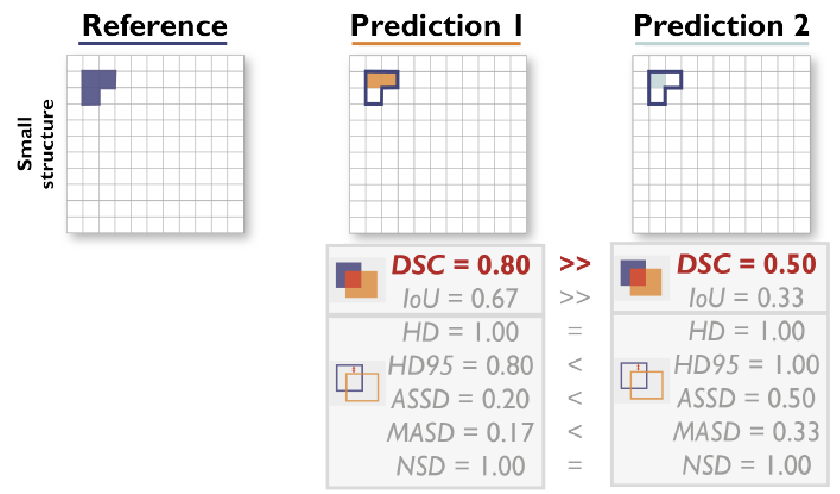
\includegraphics[width=.45\linewidth]{figures/size-b.png}}
    \subfigure{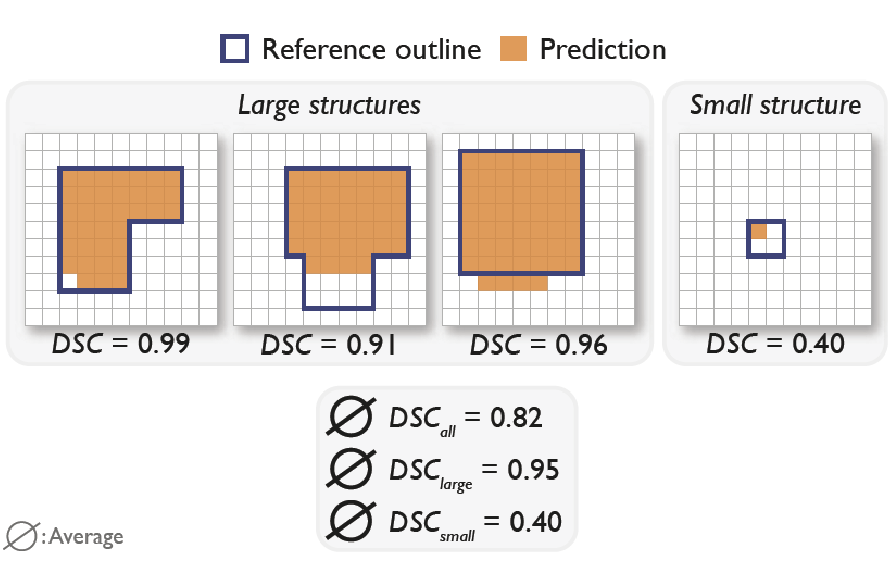
\includegraphics[width=.45\linewidth]{figures/size-c.png}}
\end{figure}

\subsubsection{Effect of structure shape}

``Common overlap-based metrics such as the Dice Similarity Coefficient (DSC) are unaware of complex structure shapes and treat Predictions 1 and 2 equally. The centerline Dice Similarity Coefficient (clDice) uncovers that Prediction 1 misses the fine-granular branches of the reference and favors Prediction 2, which focuses on the object’s center line and better captures its fine branches. This pitfall is also relevant for other overlap-based metrics''~\cite{pitfalls-in-segmentation-evaluation}

\begin{figure}[H]
    \centering
    \subfigure{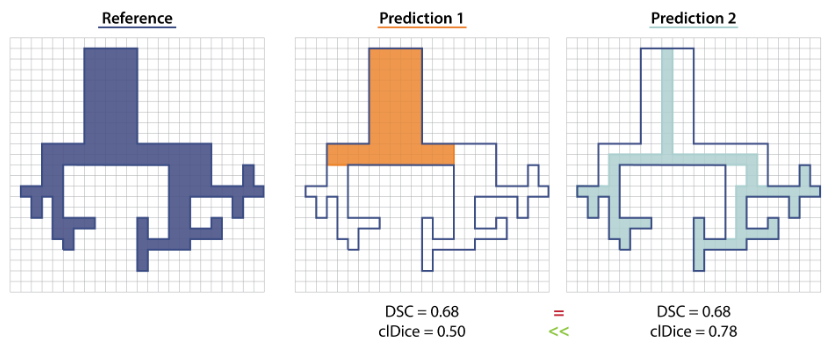
\includegraphics[width=\linewidth]{figures/shape--1.png}}
    \caption{Extended Data Fig. Sn 2.14~\cite{pitfalls-in-segmentation-evaluation}}
\end{figure}

\begin{figure}[H]
    \centering
    \subfigure{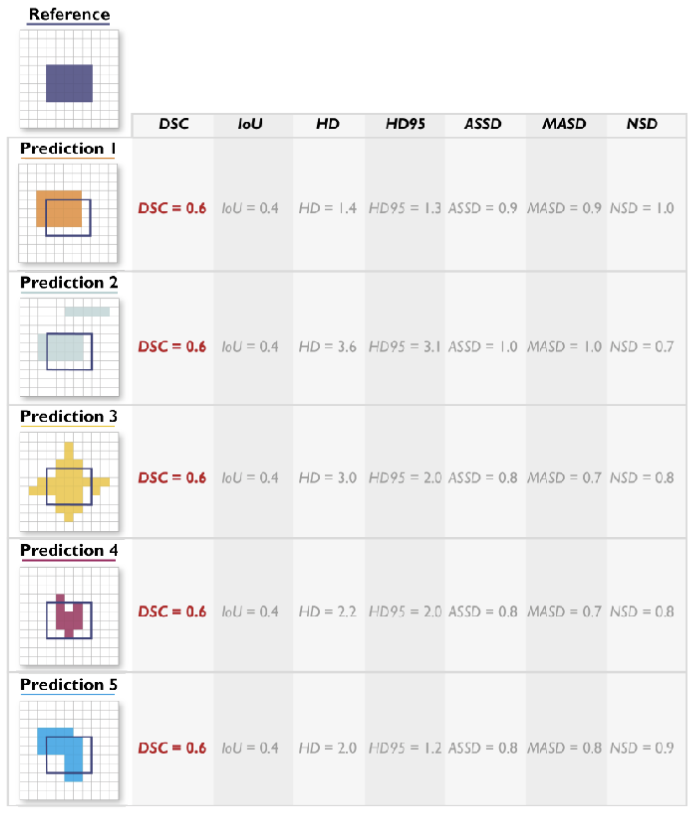
\includegraphics[width=\linewidth]{figures/shape.png}}
\end{figure}

\subsubsection{Effect of spatial alignment}

``The most common counting-based metrics are poor proxies for the center point alignment. Here, Predictions 1 and 2 yield the same Dice Similarity Coefficient (DSC) value although Prediction 1 approximates the location of the object much better''~\cite{pitfalls-in-segmentation-evaluation}. This pitfall is also reveleant for other boundary and overla-based metrics such as Boundary Intersection over Union (IoU) and Hasudorff Distance (HD).

\begin{figure}[H]
    \centering
    \subfigure{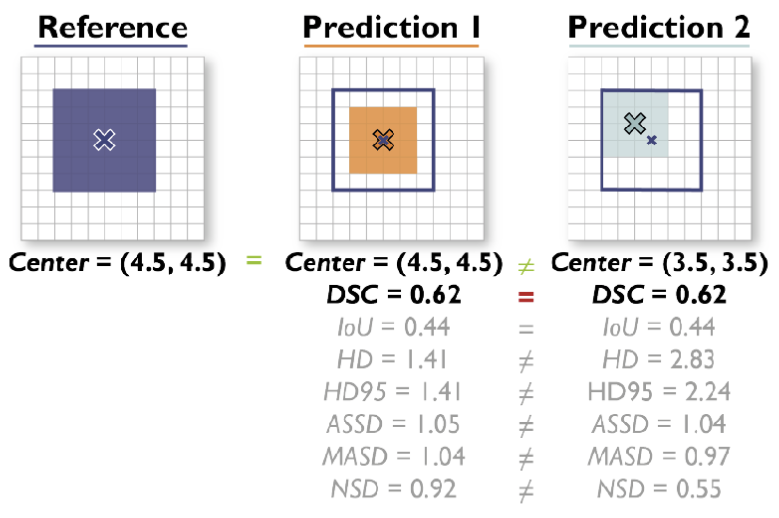
\includegraphics[width=.6\linewidth]{figures/alignment.png}}
    \caption{Extended Data Fig. SN 2.7~\cite{pitfalls-in-segmentation-evaluation}}
\end{figure}

\subsubsection{Effect of holes}

Boundary-based metrics commonly ignore the overlap between structures and are thus insensitive to holes in structures.

\begin{figure}[H]
    \centering
    \subfigure{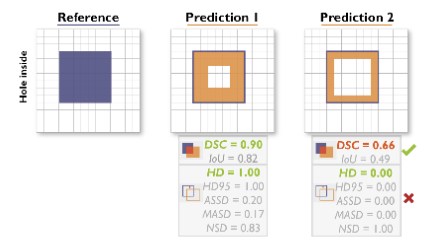
\includegraphics[width=.45\linewidth]{figures/holes-1.png}}
    \subfigure{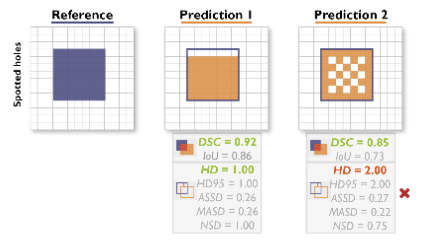
\includegraphics[width=.45\linewidth]{figures/holes-2.png}}
    \caption{Extended Data Fig. SN 2.6~\cite{pitfalls-in-segmentation-evaluation}}
\end{figure}

\subsubsection{Effect of Annotation noise}

\begin{figure}[H]
    \centering
    \subfigure{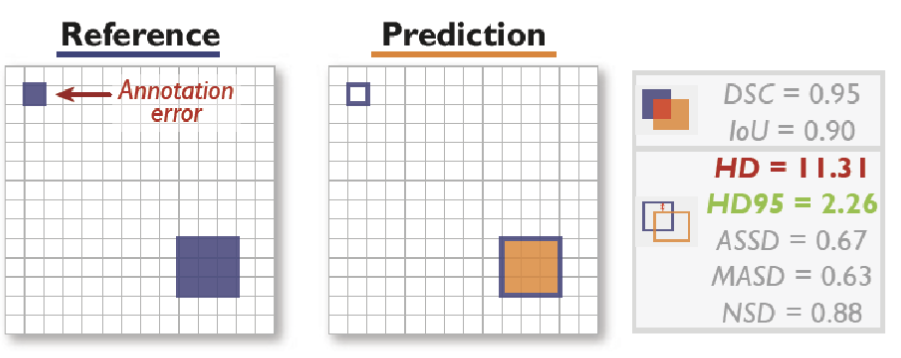
\includegraphics[width=.45\linewidth]{figures/noise-a.png}}
    \subfigure{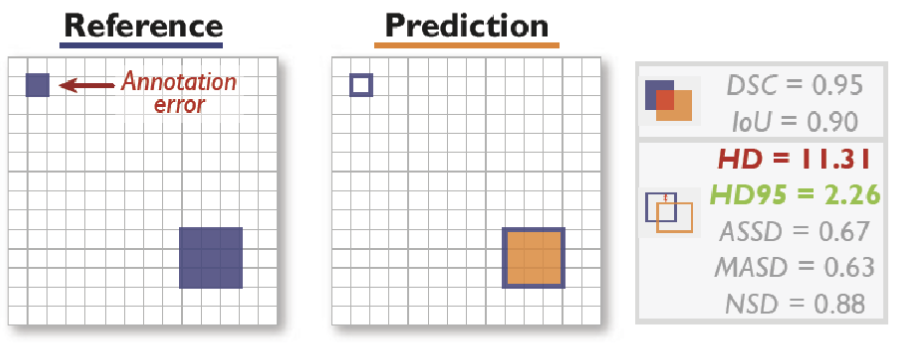
\includegraphics[width=.45\linewidth]{figures/noise-b.png}}
\end{figure}

\subsubsection{Effect of empty labelmaps}

\begin{figure}[H]
    \centering
    \subfigure{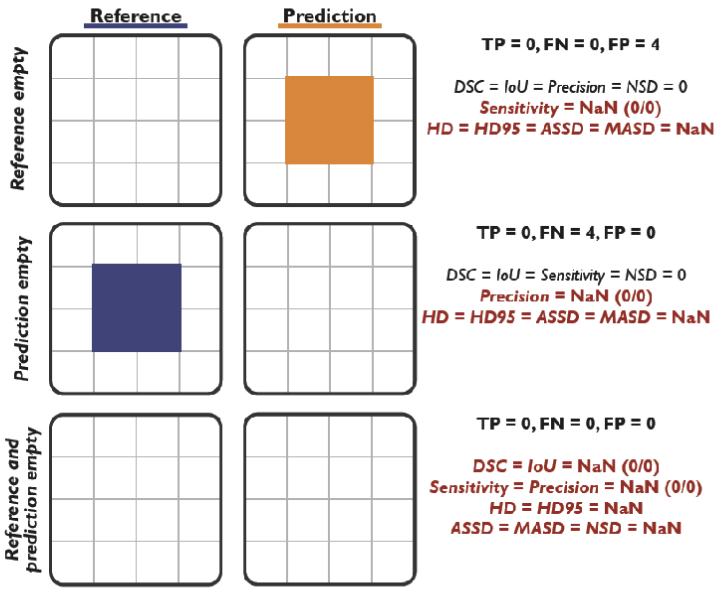
\includegraphics[width=.6\linewidth]{figures/empty-label-map-1.png}}
\end{figure}

\subsubsection{Effect of resolution}

Differences in the grid size (resolution) of an image highly influence the image and the reference annotation (dark blue shape (reference) vs. pink outline (desired circle shape)), with a prediction of the exact same shape leading to different metric scores.

\begin{figure}[H]
    \centering
    \subfigure{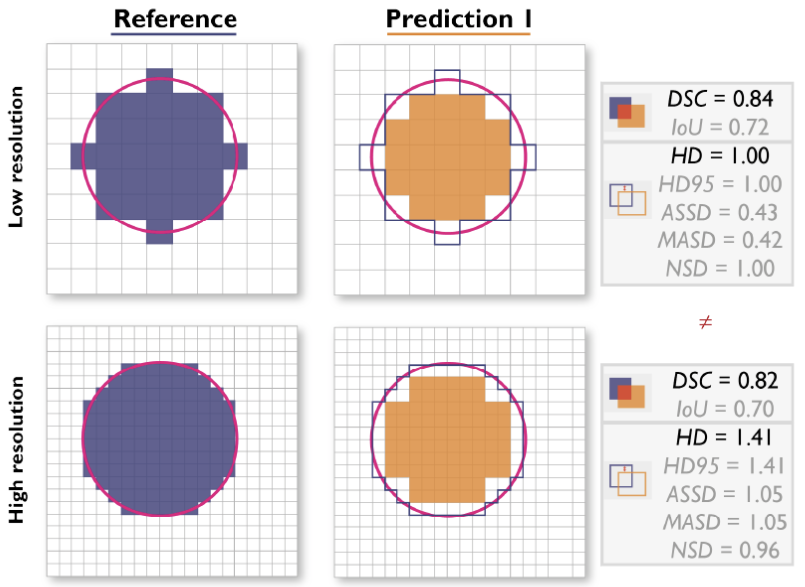
\includegraphics[width=.6\linewidth]{figures/resolution-1.png}}
    \caption{Effect of different grid sizes. Extended Data Fig. SN 2.36~\cite{pitfalls-in-segmentation-evaluation}}
\end{figure}

\subsection{Preference for oversegmentatin to undersegmentation}

The outlines of the predictions of two algorithms (Prediction 1/2) differ in only a single layer of pixels (Prediction 1: undersegmentation | smaller structure compared to eference, Prediction 2: oversegmentation | larger structure compared to reference).

If penalizing of either over- or undersegmentation is desired (unequal severity of class confusions), other metrics such as the $F_\beta$ Score provide specific penalties for either depending on the chosen hyperparameter $\beta$. This pitfall is also relevant for other overlap-based metrics such as centerline Dice Similarity Coefficient ( clDice)

\begin{figure}[H]
    \centering
    \subfigure{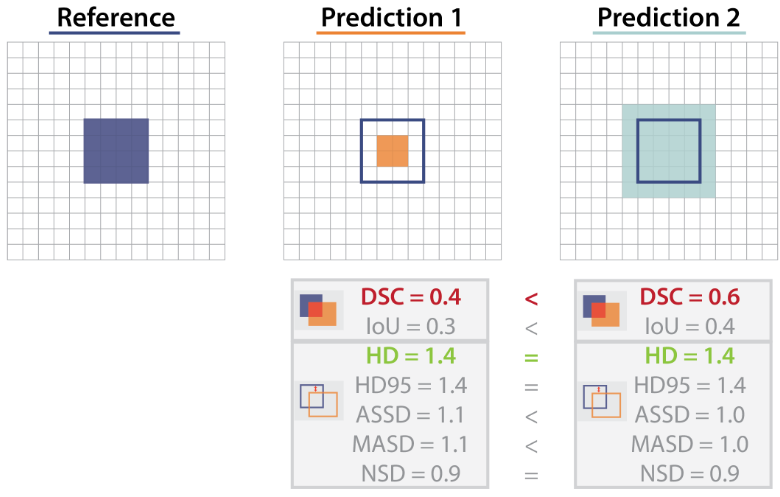
\includegraphics[width=.6\linewidth]{figures/oversegmentation.png}}
    \caption{Extended Data Fig. SN 2.10~\cite{pitfalls-in-segmentation-evaluation}}
\end{figure}

\section{Segmentation Methods}

\subsection{Intensity-based segmentation | thresholding}

By generating a histogram of values from a scan, you can choose which pixels to keep based on a threshold. When one threshold doesn't work initially, you can use multiple thresholds with upper and lower thresholds

\begin{figure}[H]
    \centering
    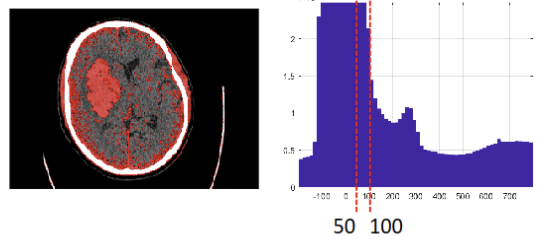
\includegraphics[width=.6\linewidth]{figures/ul-thresholding.png}
\end{figure}

\subsubsection{Advantages}

Simple and fast

\subsubsection{Disadvantages}

\begin{itemize}
    \item regions must be homogeneous and distinct
    \item difficulty in finding consistent thresholds across images
    \item leakages, isolated pixels and `rough' boundaries likely
\end{itemize}

\subsection{Region-based | region growing}

Start from (user selected) seed point(s) and grow a region according to an intensity threshold.

\begin{figure}[H]
    \centering
    \subfigure{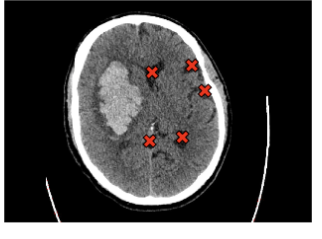
\includegraphics[width=.4\linewidth]{figures/regiongrow-1.png}}
    \subfigure{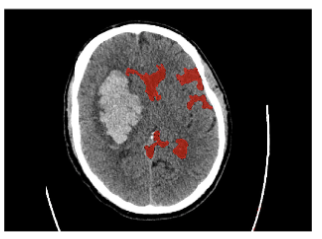
\includegraphics[width=.4\linewidth]{figures/regiongrow-2.png}}
\end{figure}

\subsubsection{Advantages}

relatively fast and yields connected regions (From a seed point)

\subsubsection{Disadvantages}

\begin{itemize}
    \item regions must be homogeneous
    \item leakages and `rough' boundaries likely
    \item requires (user) input for seed points
\end{itemize}

\subsection{Atlas-based segmentation}

An atlas is some kind of prototype or examplar of the anatomy that we want to segment, or a template of the obejct we would like to segment. 

\begin{figure}[H]
    \centering
    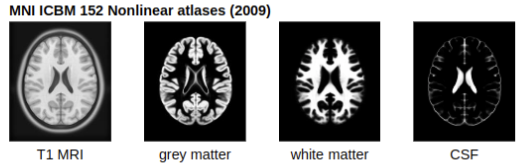
\includegraphics[width=.7\linewidth]{figures/atlas.png}
\end{figure}


Atlases usually have geometric informatino about points, curves or surfaces, or label information about voxels (Anatomical regions or function). Atlases are usually constructed from example data: single subjects or populations of subjects e.g. by averaging to produce probabilistic atlases.

The image above isn't a specific patient, but it is a statistical population average with probability maps for were brain matter is. We can use these as priors to segment other patients. 

\subsection{Segmentation using Registration}

Uses atlases to mutate and trasnform existing segmented images (or atlases) to form the same properties as the image you're trying to segment now. By using more than one image, the target image now has multiple predictions of the segmentation, and a lable fusion must occur.

\begin{figure}[H]
    \centering
    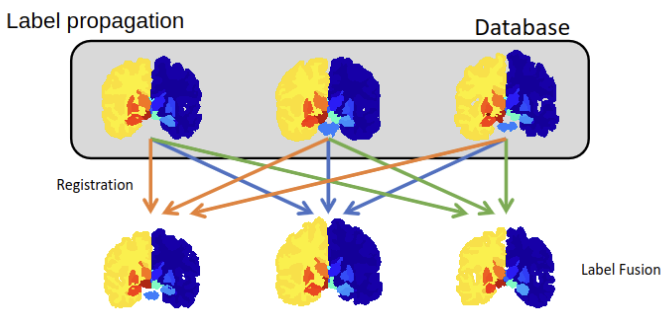
\includegraphics[width=.6\linewidth]{figures/registration.png}
\end{figure}

\subsection{Multi-Atlas Label Propagation}

\begin{figure}[H]
    \centering
    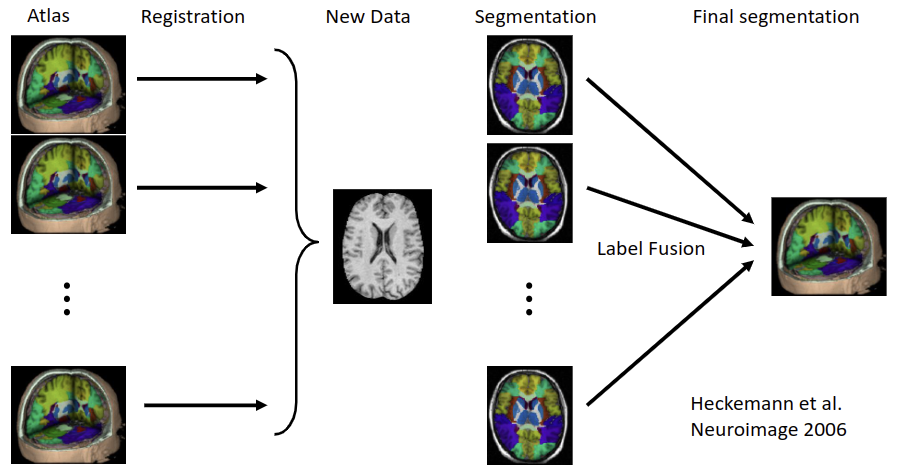
\includegraphics[width=.6\linewidth]{figures/registration-2.png}
\end{figure}

Upon fusion, it is possible to keep a probability distirbution to indicate that there was contention between different sources.

\subsubsection{Advantages}

\begin{itemize}
    \item robust and accurate (like ensembles)
    \item yields plausible segmentations
    \item fully automatic
\end{itemize}

\subsubsection{Disadvantages}

\begin{itemize}
    \item computationally expensive
    \item cannot deal well with abnormalities
    \item not suitable for tumour segmentation
\end{itemize}

\subsection{Learning-based segmentation | random forests, convolutional neural networks}

\subsubsection{Random forests}

Begin by taking different 3D views or obtain multiple contrasts of the same anatomy but in a different way (based on differen physical scans) of the same target. Afterwards, combine them into a 4D tensor, and predict a segmentaiton of the tumorous tissues. It is great because all pateints are different.

At each branch, decide a splitting criteria that will give you the best possible split amongs the data. At training, the tree tries to cluster classes together.

\begin{figure}[H]
    \centering
    \subfigure{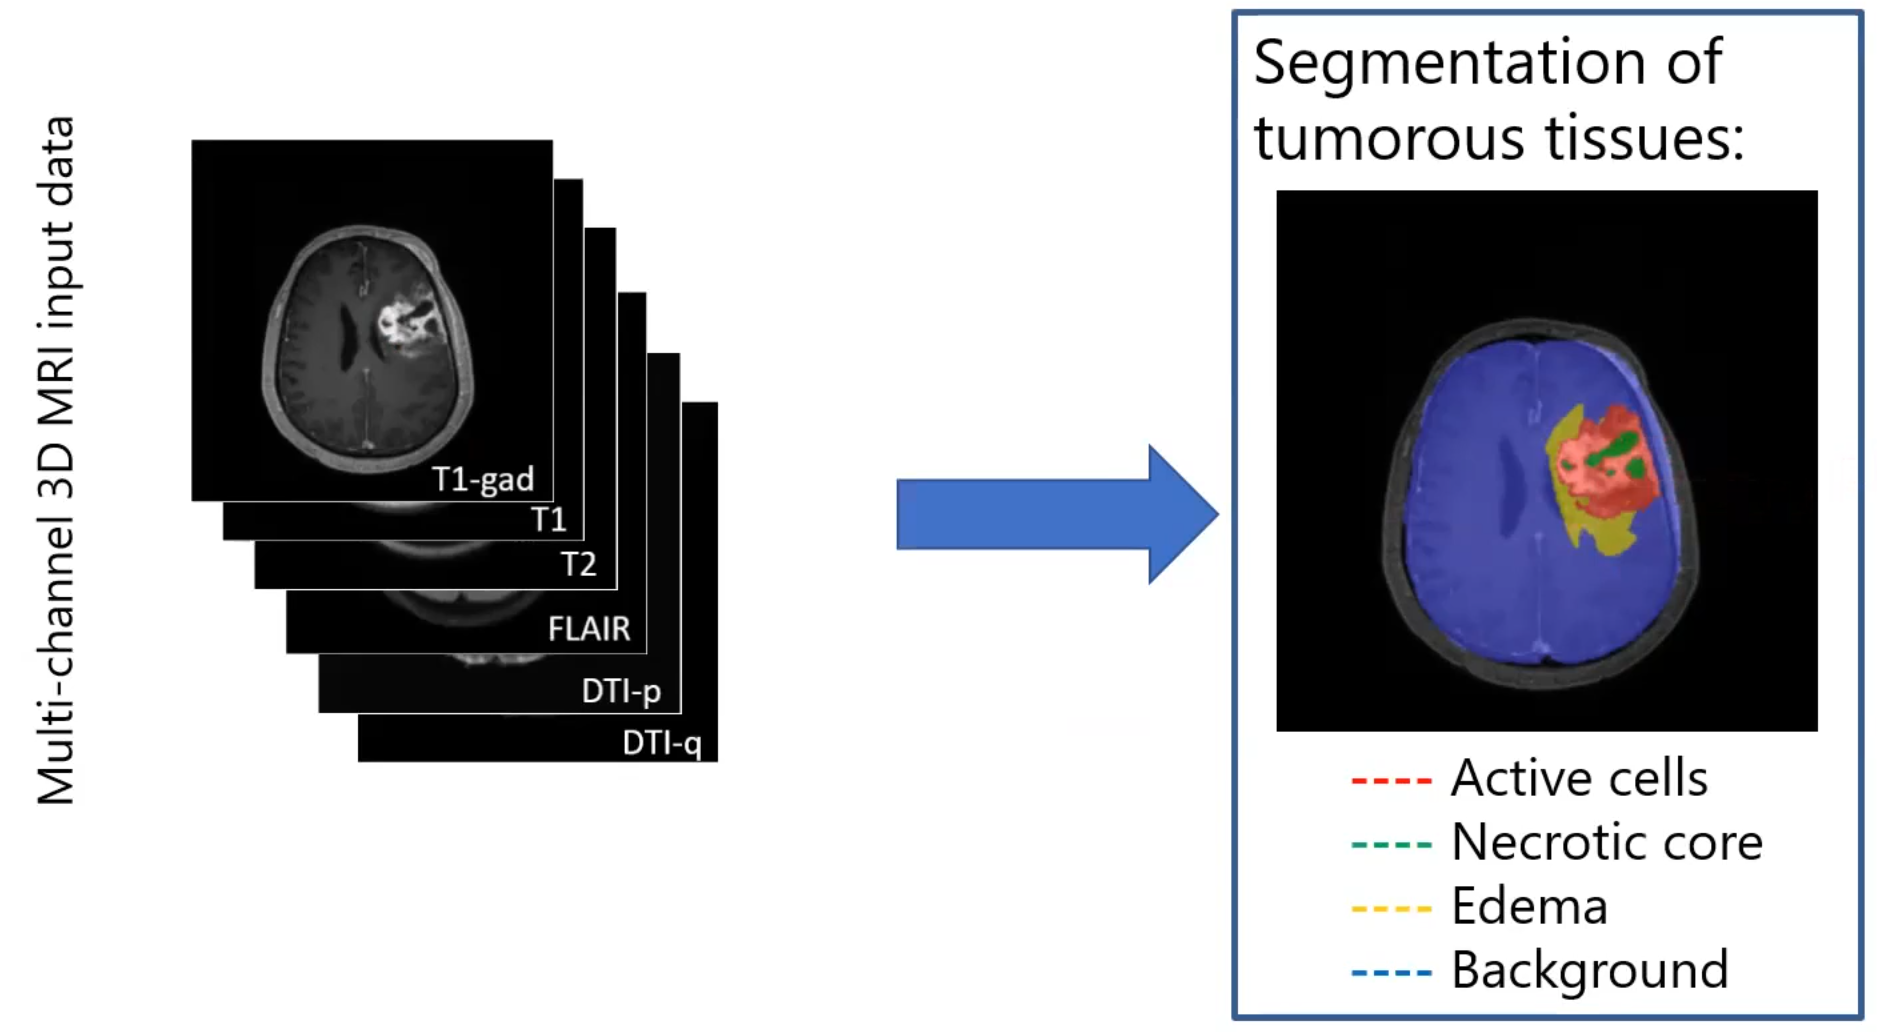
\includegraphics[width=.6\linewidth]{figures/random-forests.png}}
    \subfigure{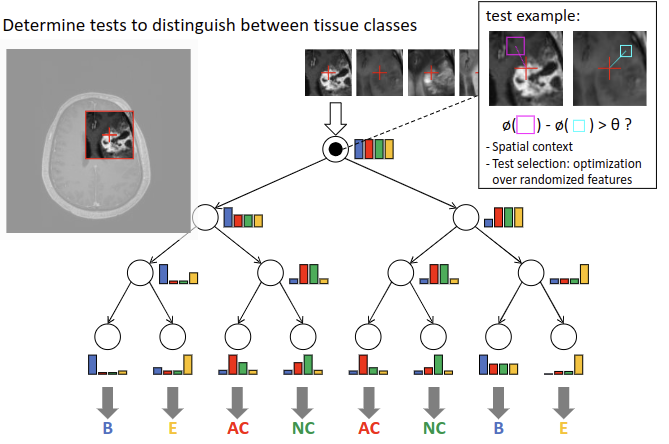
\includegraphics[width=.6\linewidth]{figures/random-forests-2.png}}
\end{figure}

\href{https://www.doc.ic.ac.uk/~bglocker/pdfs/zikic2012miccai.pdf}{paper1} and 
\href{https://www.doc.ic.ac.uk/~bglocker/pdfs/zikic2012brats.pdf}{paper2}

\subsubsection{Advantages}

\begin{itemize}
    \item ensemble classifiers are robust and accurate
    \item computationally efficient (can run in parallel)
    \item fully automatic
\end{itemize}

\subsubsection{Disadvantages}

\begin{itemize}
    \item shallow model, no hierarchical features
    \item no guarantees on connectedness
\end{itemize}

\section{Segmentation via Dense Classification}

\subsection{LeNet}

\begin{figure}[H]
    \centering
    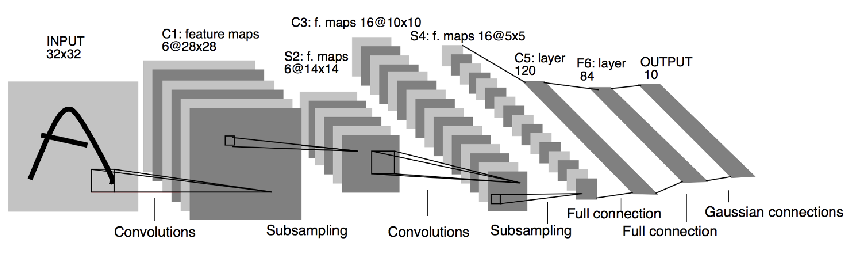
\includegraphics[width=\linewidth]{figures/LeNet.png}
\end{figure}

\lstinputlisting[language=python,firstline=1,lastline=39]{code/LeNet.py}

\subsubsection{Fully convolutional LeNet}

Pay attention to line 19 onwards. If we wanted to translate the network into a fully convolutional LeNet:

\lstinputlisting[language=python,firstline=1,lastline=34]{code/LeNet-fullyconnected.py}

\begin{figure}[H]
    \centering
    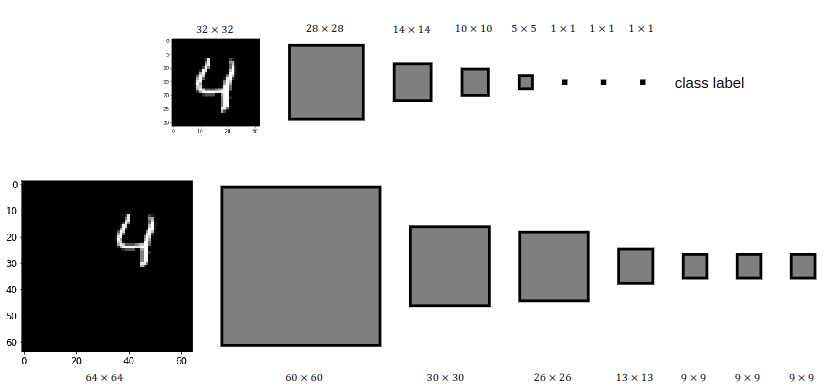
\includegraphics[width=.8\linewidth]{figures/LeNet-before-after.png}
\end{figure}

We go beyond classification. If we're given a 64x64 image, at the end of the network, we get an output feature-map. 

\begin{figure}[H]
    \centering
    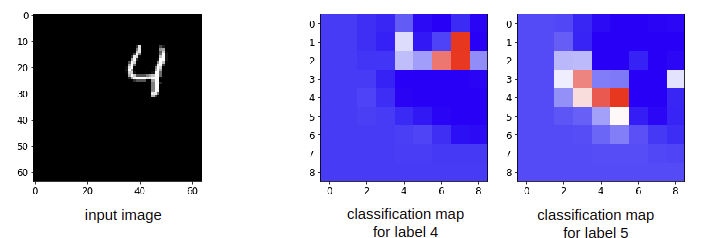
\includegraphics[width=.8\linewidth]{figures/LeNet-feature-map.png}
\end{figure}

The classication maps can be used to localise where it is, and that there is a number there (a 4). The 5, is garbage becuase there is a 5. This input is scaled up through up-sampling (Section~\ref{sect:upsample})


\section{Encoder-Decoder Networks}

\begin{figure}[H]
    \centering
    \subfigure{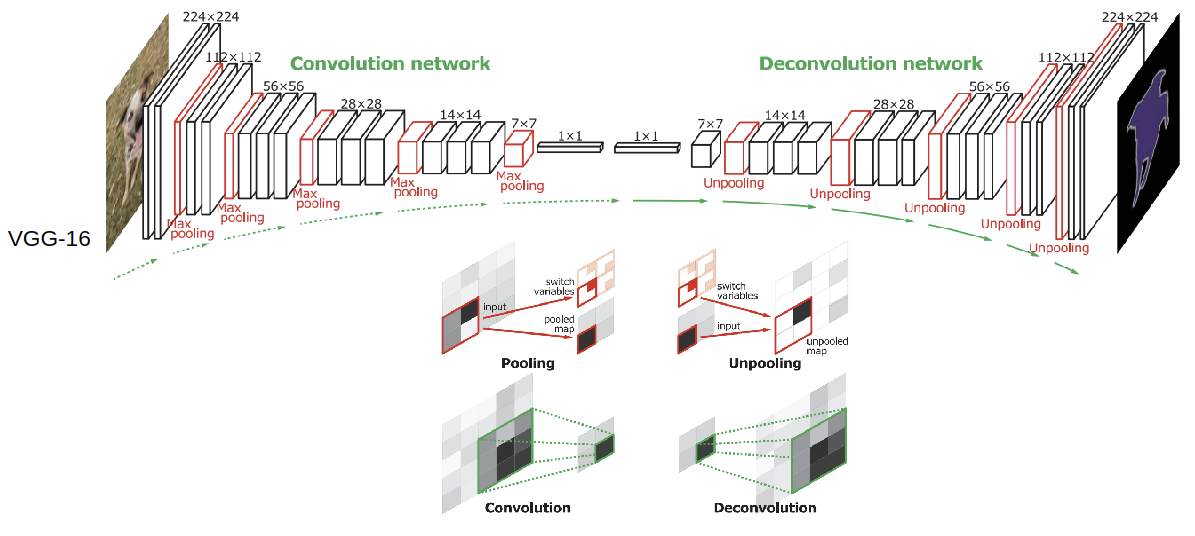
\includegraphics[width=.7\linewidth]{figures/encoder-decoder.png}}
\end{figure}

\begin{figure}[H]
    \centering
    \subfigure{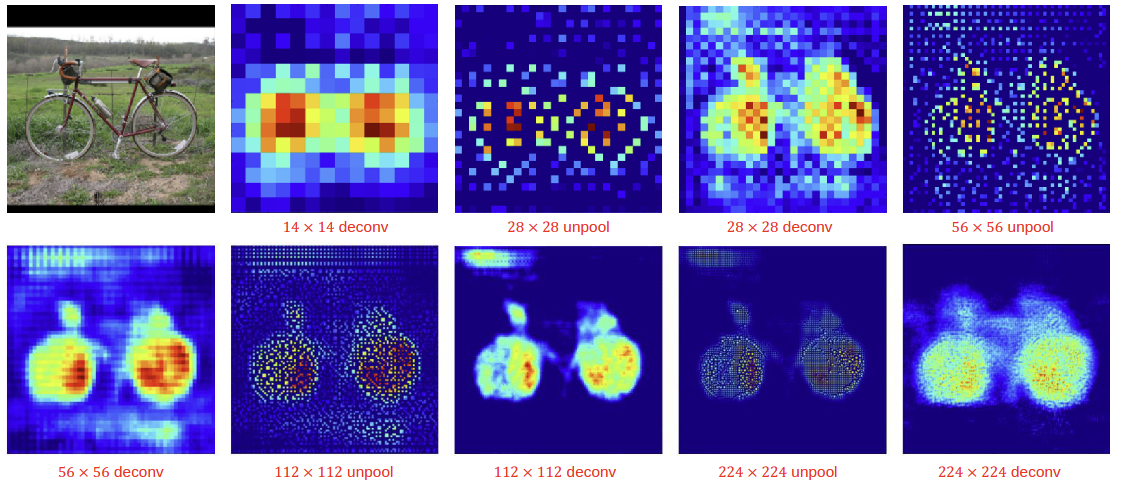
\includegraphics[width=.7\linewidth]{figures/encoder-decoder-2.png}}
\end{figure}

The idea is to take a really low level representation of an image and try to upsample it back to its original resolution. This is what the U-Net is trying to achieve.

\subsection{U-Net}

\begin{figure}[H]
    \centering
    \subfigure{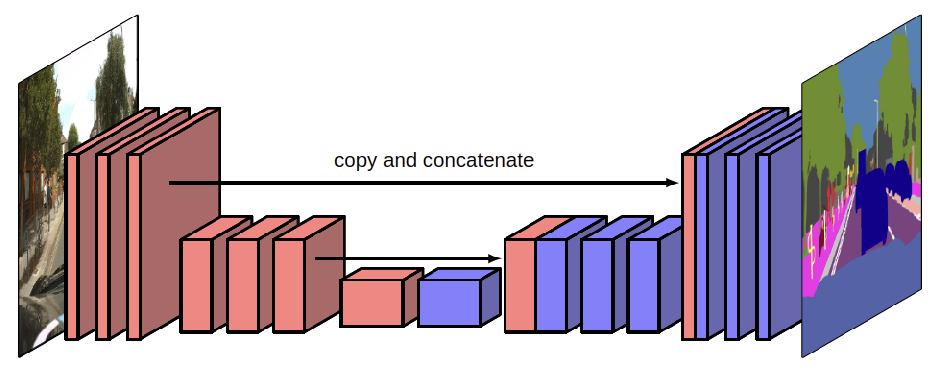
\includegraphics[width=.7\linewidth]{figures/u-net.png}}
\end{figure}

\subsubsection{Upsampling}\label{sect:upsample}

\begin{figure}[H]
    \centering
    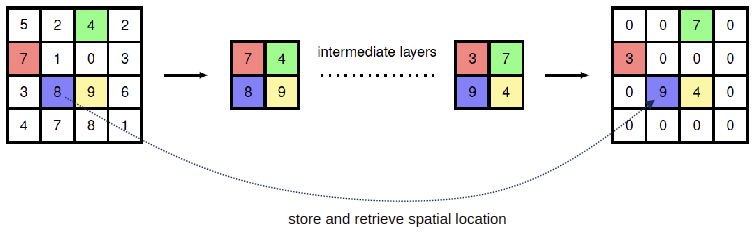
\includegraphics[width=.8\linewidth]{figures/upsampling.png}
\end{figure}

\subsubsection{Convolutions}

\begin{figure}[H]
    \centering
    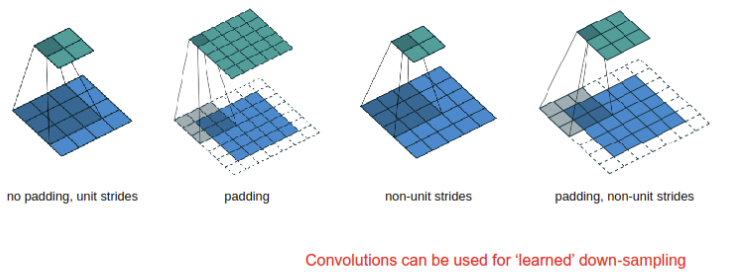
\includegraphics[width=.8\linewidth]{figures/convolutions.png}
\end{figure}

\href{https://github.com/vdumoulin/conv_arithmetic}{link}

\subsubsection{Transpose convolutions}

\begin{figure}[H]
    \centering
    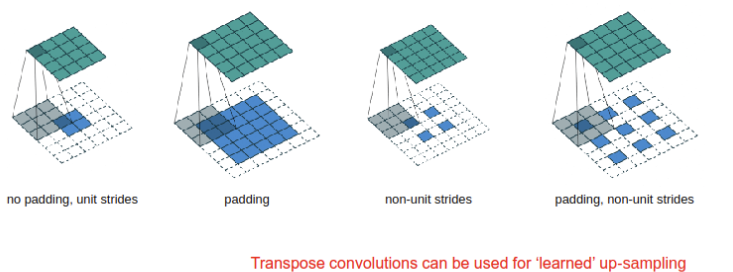
\includegraphics[width=.8\linewidth]{figures/transpose-convolutions.png}
\end{figure}

\href{https://github.com/vdumoulin/conv_arithmetic}{link}

\subsubsection{Dilated convolutions}

\begin{figure}[H]
    \centering
    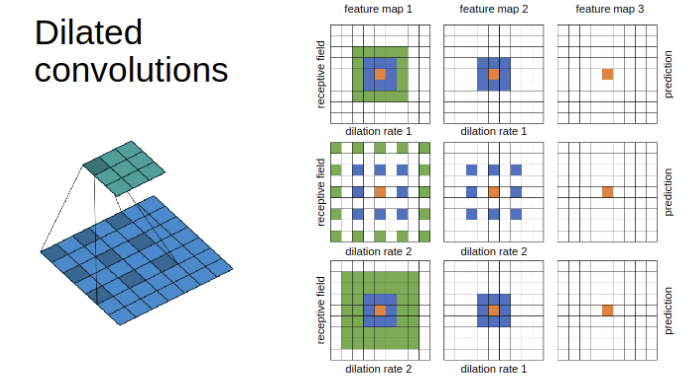
\includegraphics[width=.8\linewidth]{figures/dilated-convolutions.png}
\end{figure}

\href{https://arxiv.org/abs/1511.07122v3}{link}

\subsubsection{Atrous spatial pyramid pooling}

\begin{figure}[H]
    \centering
    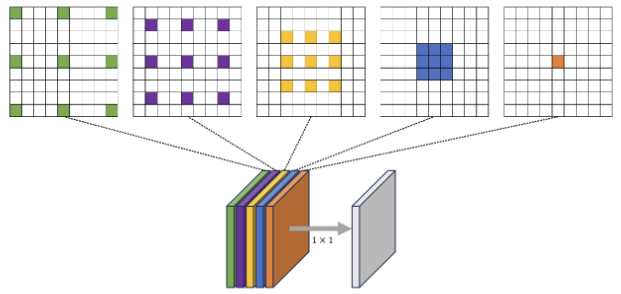
\includegraphics[width=.8\linewidth]{figures/atrous-spatial-pooling.png}
\end{figure}

\href{https://arxiv.org/abs/1606.00915}{link}

\subsubsection{Padding effects}

\begin{figure}[H]
    \centering
    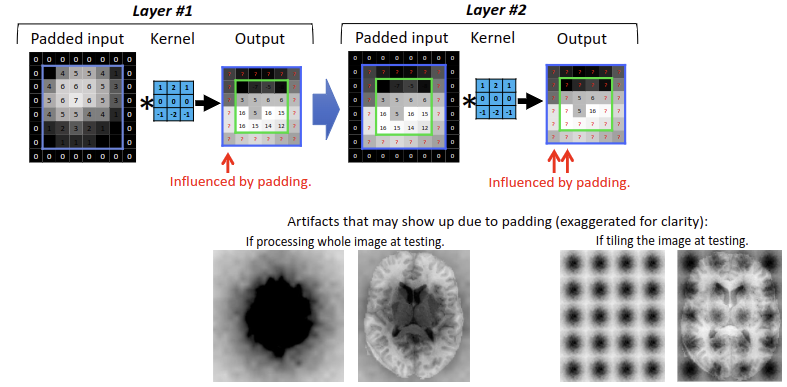
\includegraphics[width=.8\linewidth]{figures/padding-effects.png}
\end{figure}

the padding may propogate values in the features, or if we used tiling or sliding window appraoch, we may get a repeating pattern.

\subsubsection{Multi-scale processing}

\begin{figure}[H]
    \centering
    \fbox{\includegraphics[page=129, trim=0cm 0cm 0cm 0cm, clip=true, width=\linewidth]{02 - Image Segmentation.pdf}}
\end{figure}

the idea of not using a decoder that given an input patch, we process it (without maxpooling) by applying convolutional layers and then we have the kernel of fully connected layers. Here, we have a receptive field, i.e. how much information we can see. The solution here is to take another network and process in paralell, the iamge at a lower resolution. Here we can see more spatial context.

\begin{figure}[H]
    \centering
    \fbox{\includegraphics[page=130, trim=0cm 0cm 0cm 0cm, clip=true, width=\linewidth]{02 - Image Segmentation.pdf}}
\end{figure}

\subsection{Vision trasnformers}

\begin{figure}[H]
    \centering
    \fbox{\includegraphics[page=134, trim=0cm 0cm 0cm 0cm, clip=true, width=\linewidth]{02 - Image Segmentation.pdf}}
\end{figure}



\begin{figure}[H]
    \centering
    \fbox{\includegraphics[page=135, trim=0cm 0cm 0cm 0cm, clip=true, width=\linewidth]{02 - Image Segmentation.pdf}}
\end{figure}

\begin{figure}[H]
    \centering
    \fbox{\includegraphics[page=136, trim=0cm 0cm 0cm 0cm, clip=true, width=\linewidth]{02 - Image Segmentation.pdf}}
\end{figure}

\begin{figure}[H]
    \centering
    \fbox{\includegraphics[page=137, trim=0cm 0cm 0cm 0cm, clip=true, width=\linewidth]{02 - Image Segmentation.pdf}}
\end{figure}

\begin{figure}[H]
    \centering
    \fbox{\includegraphics[page=138, trim=0cm 0cm 0cm 0cm, clip=true, width=\linewidth]{02 - Image Segmentation.pdf}}
\end{figure}


\printbibliography
\addcontentsline{toc}{section}{Bibliography}

\end{document}